\chapter{Overture}
This book contains the central elements of my physics degree. It is written during my stidues and finished after my PhD. Roughly speaking the book is divided into five parts; classical mechanics (large object moving at $v\ll c$), relativistic mechanics (large objects moving at $v\sim c$), quantum mechanics (small objects moving at $v\ll c$), quantum field theory (small objects moving at $v\sim c$) and lastly statitics.
\begin{figure}[H]
	\captionsetup{width=1\textwidth}
	\centering
	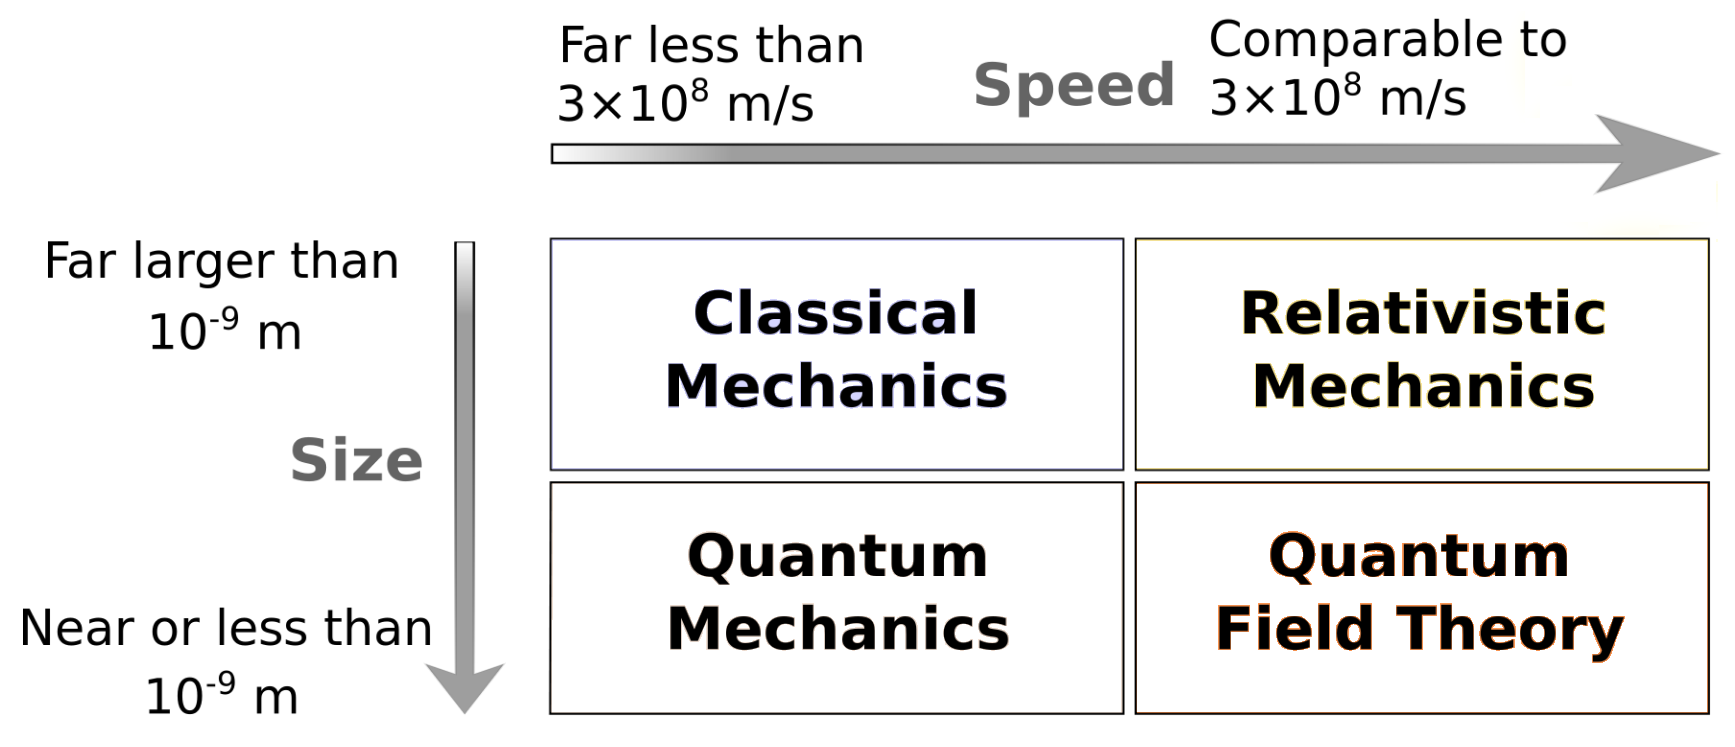
\includegraphics[width=0.6\textwidth]{figures/ov}
\end{figure}

\section{Notation}
\label{sec:notation}
\paragraph{Units:}
\index{Natural units}
Since this book will cover many different fields of physics will vary slightly throughout. As a rule of thumb; In the non-relativistic limit ($v\ll c$) SI units will be employed whereas in the relativistic limit ($v\simeq c$) natural units ($\hbar=k_B=c=1$) will be utilized. 

\paragraph{Vectors:}
Apart from the statistics part, a three vector will be denoted by a vector arrow, eg. $\vec{x}$, whereas a four vector will most often have no specific notation, eg. $x=x^\mu\doteq (x^0,x^1,x^2,x^3)^T$. A four vector with index up, eg. $x^\mu$, is a contravariant vector whereas a four vector with index down, eg. $x_\mu$, is a covariant vector (a deeper explanation and definition is found in section \ref{sec:lor}).

\paragraph{Derivatives:}
The partial derivative is denoted by $\partial_\mu= \frac{\partial}{\partial x^\mu}$ and the (Minkowski space) d'Alembertian is $\square=\partial_\mu\partial^\mu=\partial_0^2-\vec{\nabla}^2$. The symbol $\breve{\partial}_\mu$ is defined by $f\breve{\partial}_\mu g=f\partial_\mu g-(d_\mu f)g$.

\paragraph{Metric:}$\eta^{(qft)}_{\mu\nu} \doteq diag(1,-1,-1,-1)$ will be used in quantum field theory\footnote{Such that $x\cdot x=x_{(0)}x^{(0)}-(x_{(1)}x^{(1)}+x_{(2)}x^{(2)}+x_{(3)}x^{(3)})$.} and $\eta^{(sr)}_{\mu\nu}\doteq diag(-1,1,1,1)$ will be used in special relativity\footnote{Such that $x\cdot x=-x_{(0)}x^{(0)}+(x_{(1)}x^{(1)}+x_{(2)}x^{(2)}+x_{(3)}x^{(3)})$.}. Under normal conditions it will be quite clear which metric is used, and so the superscripts will be suppressed. A generic metric, valid in spaces which differ from Minkowski (special relativity), is denoted by $g_{\mu\nu}$. Often $g_{\mu\nu}$ and $\eta_{\mu\nu}$ will be used interchangeably.

\paragraph{Dirac matrices:} 
\index{Dirac matrices} 
Dirac matrices, $\gamma^\mu$, satisfy

\begin{equation}
	\{\gamma^\mu,\gamma^\nu\}=\gamma^\mu\gamma^\nu+\gamma^\nu\gamma^\mu=2\eta^{\mu\nu}.
\end{equation} 
Therefore $(\gamma^{0})^2=I\doteq1$ and $(\gamma^i)=-I\doteq -1$. $\gamma^0$ is hermitian whereas $\gamma^i$ is anti-hermitian, i.e.

\begin{equation}
	(\gamma^0)^\dagger=\gamma^0, \quad (\gamma^i)^\dagger=-\gamma^i \rightleftarrows (\gamma^\mu)^\dagger=\gamma^0\gamma^\mu\gamma^0,
\end{equation} 
where $\dagger=*T$ in matrix notation. The Dirac matrices satisfy the contraction identities

\begin{equation}
	\begin{split}
		\gamma^\mu\gamma_\mu&=\eta_{\mu\nu}\gamma^\mu\gamma^\nu=\frac{1}{2}g_{\mu\nu}\{\gamma^\mu,\gamma^\nu\}=\eta_{\mu\nu}\eta^{\mu\nu}=4,\\
		\gamma^\mu\gamma^\nu\gamma_\mu&=-2\gamma^\nu,\\
		\gamma^\mu\gamma^\nu\gamma^\alpha\gamma_\mu&=4\eta^{\nu\alpha},\\
		\gamma^\mu\gamma^\nu\gamma^\alpha\gamma^\beta\gamma_\mu&=-2\gamma^\beta\gamma^\alpha\gamma^\nu,\\
	\end{split}
\end{equation} 
where Einstein summations is used (repeated indices are summed implicitly). The matrix $\gamma^5$ is defined as follows

\begin{equation}
	\gamma^5\equiv i\gamma^0\gamma^1\gamma^2\gamma^3,
\end{equation} 
where

\begin{equation}
	(\gamma^5)^2=I\doteq 1, \quad (\gamma^5)^\dagger=\gamma^5, \quad \{\gamma^5,\gamma^\mu\}=0.
\end{equation} 
The commutator of the Dirac matrices is defined as follows

\begin{equation}
	[\gamma^\mu,\gamma^\nu]=\gamma^\mu\gamma^\nu-\gamma^\nu\gamma^\mu\equiv -2i\sigma^{\mu\nu},
\end{equation} 
where $\sigma^{\mu\nu}$ is a rank 2 tensor. The Dirac matrices obey the following trace identities

\begin{equation}
	\begin{split}
		Tr(I)&=Tr(1)=4,\\
		Tr(\gamma^\mu)&=0,\\
		Tr(\gamma^5)&=0,\\
		Tr(\text{odd $\#$ of $\gamma$'s})&=0,\\
		Tr(\gamma^\mu\gamma^\nu)&=4\eta^{\mu\nu},\\
		Tr(\gamma^\mu\gamma^\nu\gamma^\alpha\gamma^\beta\dots)&=Tr(\dots\gamma^\beta\gamma^\alpha\gamma^\nu\gamma^\mu),\\
		Tr(\gamma^5\gamma^\mu\gamma^\nu)&=0,\\
		Tr(\gamma^\mu\gamma^\nu\gamma^\alpha\gamma^\beta)&=4(\eta^{\mu\nu}\eta^{\alpha\beta}-\eta^{\mu\alpha}\eta^{\nu\beta}+\eta^{\mu\beta}\eta^{\nu\alpha}),\\
		Tr(\gamma^5\gamma^\mu\gamma^\nu\gamma^\alpha\gamma^\beta)&=-4i\varepsilon^{\mu\nu\alpha\beta},\\
	\end{split}
\end{equation} 

where $\varepsilon^{\dots}$ is the Levi-Civita tensor which obeys

\begin{equation}
	\begin{split}
		\varepsilon^{0123}&=1\\
		\varepsilon^{0132}&=-1\\
		\varepsilon^{\mu\nu\alpha\beta}\varepsilon_{\mu\nu\alpha\beta}&=-24,\\
		\varepsilon^{\mu\nu\alpha\beta}\varepsilon_{\mu\nu\alpha\sigma}&=-6\delta^\beta_{\,\,\, \sigma},\\
		\varepsilon^{\mu\nu\alpha\beta}\varepsilon_{\mu\nu\rho\sigma}&=-2(\delta^\alpha_{\,\,\, \rho}\delta^\beta_{\,\,\, \sigma}-\delta^\alpha_{\,\,\, \sigma}\delta^\beta_{\,\,\, \rho}).\\
	\end{split}
\end{equation} 
The Dirac matrices can be represented by several, equivalent, matrix representations (there is an ambiguity in the definition from the Dirac equation). Two often used representations are the Weyl representation (also called the chiral representation) and the standard representation

\begin{equation}
	\begin{split}
		&\text{Weyl rep.:} \quad \gamma^0\doteq \begin{bmatrix}
			0 & 1 \\
			1 & 0 \\
		\end{bmatrix}, \quad \gamma^i\doteq\begin{bmatrix}
			0 & \sigma^i \\
			-\sigma^i & 0 \\
		\end{bmatrix}, \quad \gamma^5\doteq\begin{bmatrix}
			-1 & 0 \\
			0 & 1 \\
		\end{bmatrix},\\
		&\text{Std. rep.:} \quad \gamma^0\doteq \begin{bmatrix}
			1 & 0 \\
			0 & -1 \\
		\end{bmatrix}, \quad \gamma^i\doteq\begin{bmatrix}
			0 & \sigma^i \\
			-\sigma^i & 0 \\
		\end{bmatrix}, \quad \gamma^5\doteq\begin{bmatrix}
			0 & 1 \\
			1 & 0 \\
		\end{bmatrix}.\\
	\end{split}
\end{equation} 
The above matrices are in block diagonal form. The Dirac matrices are $4\times 4$ matrices, so each block is $2\times 2$. $\sigma^i$ are called the Pauli matrices and are defined viz

\begin{equation}
	\sigma^1\doteq \begin{bmatrix}
		0 & 1\\
		1 & 0 \\
	\end{bmatrix}, \quad \sigma^2\doteq \begin{bmatrix}
		0 & -i\\
		i & 0 \\
	\end{bmatrix}, \quad \sigma^3\doteq \begin{bmatrix}
		1 & 0\\
		0 & -1 \\
	\end{bmatrix}.
\end{equation} 
The Pauli matrices satisfy

\begin{equation}
	\sigma^i \sigma^j=\delta^{ij}+i\varepsilon^{ijk}\sigma^k.
\end{equation} 
In relation to the Pauli matrices two 4-vectors are defined

\begin{equation}
	\sigma^\mu\equiv (1,\sigma^i), \quad \bar{ \sigma}^\mu\equiv (1,-\sigma^i).
\end{equation} 

\paragraph{Slash and bar notation:}
Feynman slash-notation is defined by

\begin{equation}
	\slashed A \equiv A_\mu\gamma^\mu=\gamma^\mu A_\mu=\gamma_\mu A^\mu=A^\mu\gamma_\mu.
\end{equation} 
Often the partial derivative will appear in slashed notation, i.e. $\slashed \partial =\gamma^\mu\partial _\mu$. The barred notation is defined by

\begin{equation}
	\bar{A}=A^\dagger \gamma^0_{Weyl},
\end{equation} 
where it is clear that the $\gamma^0$ to be used is only the one from the Weyl representation. The function of this $\gamma^0$ is to swap the upper and lower components in a $2\times 1$ matrix and this is what is needed. The $\gamma^0$ from the standard representation does not do this. Note however that henceforth the subscript on the $\gamma^0$ will be omitted and it it understood that for barred quantities (other than $\bar{\sigma}$ which is poorly defined in this notation) the relevant $\gamma^0$ is the one from the Weyl representation.

\paragraph{Dirac Spinors:} The Dirac spinors are defined as follows

\begin{equation}
	\begin{split}
		&u^s(\vec{p})=\begin{bmatrix}
			\sqrt{p\cdot \sigma}\xi^s\\
			\sqrt{p\cdot \bar{\sigma}}\xi^s\\
		\end{bmatrix}, \quad \bar{u}^s(\vec{p})=\begin{bmatrix}
			\xi^{\dagger s}\sqrt{p\cdot \sigma} & \xi^{\dagger s}\sqrt{p\cdot \bar{\sigma}}
		\end{bmatrix}\gamma^0, \\
		&v^{s'}(\vec{k})=\begin{bmatrix}
			\sqrt{k\cdot \sigma} \eta^{s'}\\
			-\sqrt{k\cdot \bar{\sigma}}\eta^{s'}
		\end{bmatrix}, \quad \bar{v}^{s'}(\vec{k})=\begin{bmatrix}
			\eta^{\dagger s'}\sqrt{k\cdot \sigma} & -\eta^{\dagger s'}\sqrt{k\cdot \bar{\sigma}}
		\end{bmatrix}\gamma^0,
	\end{split}
\end{equation} 
where\footnote{The identity $\xi^{\dagger s'}\eta^{s}=\delta^{ss'}$ encourages the identification $\xi=\eta$, just as \citet{Peskin1995}[p. 65] has done.} $\xi^{\dagger s'}\xi^s=\delta^{ss'}$, $\eta^{\dagger s'}\eta^s=\delta^{ss'}$, $\xi^{\dagger s'}\eta^{s}=\delta^{ss'}$ and the $\sqrt{p\cdot \sigma}$-like expressions are to be understood as the square root of the positive eigenvalue of the matrix $p\cdot \sigma$. Hence, the $\sqrt{p\cdot \sigma}$-like expressions are numbers and can be moved around as such. The $\sqrt{p\cdot \sigma}$-like expressions obey

\begin{equation}
	\begin{split}
		&\sqrt{p\cdot \sigma}=\sqrt{p^0-\vec{\sigma}\cdot\vec{p}}=\sqrt{eigenvals(p^0I-\vec{\sigma}\cdot\vec{p})}\\
		&\qquad \,\,\,\, =\begin{bmatrix}
			\sqrt{p^0-|\vec{p}|} & 0 \\
			0 & \sqrt{p^0+|\vec{p}|}\\
		\end{bmatrix},\\
		&\sqrt{p\cdot \bar{\sigma}}=\sqrt{p^0+\vec{\sigma}\cdot\vec{p}}=\sqrt{eigenvals(p^0I+\vec{\sigma}\cdot\vec{p})}\\
		&\qquad \,\,\,\, =\begin{bmatrix}
			\sqrt{p^0+|\vec{p}|} & 0 \\
			0 & \sqrt{p^0-|\vec{p}|}\\
		\end{bmatrix}.
	\end{split}
\end{equation} 
Since there are several eigenvalues which one is taken depends on the vector ($\xi,\eta$) which is multiplied (see \citealt{Lancaster2014}[p. 329]). For the Dirac spinors
\begin{equation}
	\begin{split}
		&u^{\dagger s}(\vec{p})u^{s'}(\vec{k})=\begin{cases}
			2p^0\delta^{ss'} & \text{if}\quad p=k\\
			\xi^{\dagger s'}[\sqrt{p\cdot \sigma}\sqrt{k\cdot \sigma}+\sqrt{p\cdot \bar{\sigma}}\sqrt{k\cdot \bar{\sigma}}\,]\xi^{s'}& \text{if}\quad p\neq k\\  
		\end{cases},\\
		&v^{\dagger s}(\vec{p})v^{s'}(\vec{k})=\begin{cases}
			2p^0\delta^{ss'} & \text{if}\quad p=k\\
			\eta^{\dagger s'}[\sqrt{p\cdot \sigma}\sqrt{k\cdot \sigma}+\sqrt{p\cdot \bar{\sigma}}\sqrt{k\cdot \bar{\sigma}}\,]\eta^{ s'}& \text{if}\quad p\neq k\\  
		\end{cases},\\
		&\bar{u}^{s}(\vec{p})u^{s'}(\vec{k})=\begin{cases}
			2m\delta^{ss'} & \text{if}\quad p=k\\
			\xi^{\dagger s'}[\sqrt{p\cdot \sigma}\sqrt{k\cdot \bar{\sigma}}+\sqrt{p\cdot \bar{\sigma}}\sqrt{k\cdot \sigma} \,]\xi^{ s'}& \text{if}\quad p\neq k\\  
		\end{cases},\\
		&\bar{v}^{s}(\vec{p})v^{s'}(\vec{k})=\begin{cases}
			-2m\delta^{ss'} & \text{if}\quad p=k\\
			-\eta^{\dagger s'}[\sqrt{p\cdot \sigma}\sqrt{k\cdot \bar{\sigma}}+\sqrt{p\cdot \bar{\sigma}}\sqrt{k\cdot \sigma} \,]\eta^{s'} & \text{if}\quad p\neq k\\ 
		\end{cases},\\
		&\bar{u}^{s}(\vec{p})v^{s'}(\vec{k})=\begin{cases}
			0 & \text{if}\quad p=k\\
			\xi^{\dagger s}[\sqrt{p\cdot \bar{\sigma}}\sqrt{k\cdot \sigma}-\sqrt{p\cdot \sigma}\sqrt{k\cdot \bar{\sigma}} \,] \eta^{s'} & \text{if}\quad p\neq k\\  
		\end{cases},\\
		&\bar{v}^{s}(\vec{p})u^{s'}(\vec{k})=\begin{cases}
			0 & \text{if}\quad p=k\\
			\eta^{\dagger s}[\sqrt{p\cdot \sigma}\sqrt{k\cdot \bar{\sigma}}-\sqrt{p\cdot \bar{\sigma}}\sqrt{k\cdot \sigma} \,] \xi^{s'}  & \text{if}\quad p\neq k\\  
		\end{cases}.\\
	\end{split}
\end{equation} 
Spin sums

\begin{equation}
	\sum_{s=1,2}u^s(\vec{p})\bar{u}^s(\vec{p})=\slashed p+m, \quad \sum_{s=1,2}v^s(\vec{p})\bar{v}^s(\vec{p})=\slashed p-m.
\end{equation} 
The solutions to Diracs equation should also be solutions to Klein-Gordons equation. The solutions to Klein-Gordons equation are plane waves, so $\psi\propto e^{\pm ip\cdot x}$ for Diracs equation. The "$\propto$" covers over $u^s(\vec{p}), v^s(\vec{o})$ (either of them). Using solutions on this form in Diracs equation results in a reduced equation from which (see equation \eqref{orse})
\begin{equation}
	\begin{split}
		u^s(\vec{p})&=\frac{\slashed p}{m}u^s(\vec{p}),\\
		\bar{u}^s(\vec{p})&=\bar{u}^s(\vec{p})\frac{\slashed p}{m},\\
		v^s(\vec{p})&=-\frac{\slashed p}{m}v^s(\vec{p}),\\
		\bar{v}^s(\vec{p})&=-\bar{v}^s(\vec{p})\frac{\slashed p}{m},\\
	\end{split}
\end{equation} 
These expressions are formidable for reducing terms on the form $\bar{u}^s(\vec{p})\Gamma v^{s'}(\vec{k})$. The procedure is as follows

\begin{equation}
	\begin{split}
		\bar{u}^s(\vec{p})\Gamma v^{s'}(\vec{k})&=\frac{1}{2}[\bar{u}^s(\vec{p})\Gamma v^{s'}(\vec{k})+\bar{u}^s(\vec{p})\Gamma v^{s'}(\vec{k})]\\
		&=\frac{1}{2}[\bar{u}^s(\vec{p})\frac{\slashed p}{m}\Gamma v^{s'}(\vec{k})-\bar{u}^s(\vec{p})\Gamma \frac{\slashed k}{m} v^{s'}(\vec{k})]\\
		&=\dots.
	\end{split}
\end{equation} 
To proceed use the specific form of $\Gamma$ alongside commutator relations and so forth.

\paragraph{Fourier transform:}
\index{Fourier transform}
The four dimensional Fourier transform is defined by

\begin{equation}
	\begin{split}
		f(x)&=\int \frac{d^4k}{(2\pi)^4}e^{-ik\cdot x}\tilde{f}(k),\\
		\tilde{f}(k)&=\int d^4x e^{ik\cdot x}f(x),\\
	\end{split}
\end{equation} 
where $x,k$ are four vectors of position an momentum, respectively and $\int d^4x=\int dx^0dx^1dx^2dx^3$. Taking the qft metric, the three dimensional Fourier transforms are defined by

\begin{equation}
	\begin{split}
		f(\vec{x})&=\int \frac{d^3k}{(2\pi)^3}e^{+i\vec{k}\cdot \vec{x}}\tilde{f}(\vec{k}),\\
		\tilde{f}(\vec{k})&=\int d^3x e^{-i\vec{k}\cdot \vec{x}}f(\vec{x}).\\
	\end{split}
\end{equation} 
For arbitrary $n$, the $n$-dimensional Dirac delta function satisfies

\begin{equation}
	\begin{split}
		\int_{-\infty}^\infty e^{-i\omega (t-t')}d\omega &=2\pi\delta(t-t'),\\
		\int d^4x e^{i(k+p)\cdot x}&=\int dx^0 e^{-i[-(k^0+p^0)]x^0}\int d^3xe^{-i(\vec{k}+\vec{p})\cdot \vec{x}},\\
		&=(2\pi)\delta[-(k^0+p_0)](2\pi)^3\delta^{(3)}(\vec{k}+\vec{p}),\\
		&=(2\pi)^4\delta^{(4)}(k+p),\\
		\int d^nx e^{i(k+p)\cdot x}&=(2\pi)^{n}\delta^{(n)}(k+p).
	\end{split}
\end{equation} 

\paragraph{Random variables:}
\index{Random variable}
The fundamental building blocks for statistics are random variables (usually denoted by $X$ or $Y$). A random variable is a way to quantify the outcome of a generic experiment. In practice this means mapping the sample space to a line of real numbers. The random variables are manipulated by operators, the most common of which are the expectation operator, $\mathbb{E}$ and the variance operator, $Var$. The two operators obey the identities
\begin{equation}
	\begin{split}
		&\mathbb{E}[X+Y]=\mathbb{E}[X]+\mathbb{E}[Y],\\
		&\mathbb{E}[aX]=a\mathbb{E}[X],\\
		&Var[X]\equiv \mathbb{E}[(X-\mathbb{E}[X])^2]\\
		&\qquad\quad=\mathbb{E}[X^2]-(\mathbb{E}[X])^2,\\
		&Var[a+X]=Var[X],\\
		&Var[aX]=a^2Var[X],\\
		&Var[aX+bY]=a^2Var[X]+b^2Var[Y]+2abCov[X,Y],\\
		&Var[aX-bY]=a^2Var[X]+b^2Var[Y]-2abCov[X,Y],\\
	\end{split}
\end{equation}
where
\begin{equation}
	\begin{split}
		Cov[X,Y]&=\mathbb{E}[(X-\mathbb{E}[X])(Y-\mathbb{E}[Y])]\\
		&=\mathbb{E}[XY]-\mathbb{E}[X]\mathbb{E}[Y],
	\end{split}
\end{equation}
where
\begin{equation}
	\begin{split}
		&Cov[X,a]=0,\\
		&Cov[X,X]=Var[X],\\
		&Cov[X,Y]=Cov[Y,X],\\
		&Cov[aX,bY]=abCov[X,Y],\\
		&Cov[a+X,b+Y]=Cov[X,Y],\\
		&Cov[aX+bY,cW+dV]=acCov[X,W]+adCov[X,V]+bcCov[Y,W]+bdCov[Y,V].\\
	\end{split}
\end{equation}
If two observations are independent, then $\mathbb{E}[XY]=\mathbb{E}[X]\mathbb{E}[Y]$. In this case it follows that the covariance vanishes. \newline\newline
The random variables can be either discrete or continuous. The random variable is discrete if the outcomes are countable, and continuous otherwise. Both discrete and continuous random variables are described by a probability function (PMF or PDF) and a cumulative function (CMF or CDF).

\paragraph{Discrete Random Variables}
In the case that the random variable, $X$, is discrete, the PMF will equal the point probability
\begin{equation}
	f(x_i)=\mathbb{P}(X=x_i),
	\label{eq1}
\end{equation} 
where
\begin{equation}
	f(x_i)>0\wedge \sum_{i=1}^{n}f(x_i)=1.
	\label{eq2}
\end{equation}
The CMF is an equivalent representation of data which is defined as
\begin{equation}
	F(x)=\mathbb{P}(X\leq x)=\sum_{x_i\leq x}f(x_i),
\end{equation}
where $0\leq F(x)\leq 1$. In the discrete case the expectation value and variance are defined viz.
\begin{equation}
	\mathbb{E}[X]=\sum_{x_i\leq x}x_if(x_i)
	,\qquad 
	Var[X]=\sum_{x_i\leq x}(x_i-\mu)^2f(x_i).
\end{equation}

\paragraph{Continuous Random Variables}
In the case that the random variable, $X$, is continuous the point probability will vanish since now the integral of the PDF must be unity, i.e. 
\begin{equation}
	\int_{-\infty }^{\infty }dx f(x)=1.
\end{equation}
Since the function integrated over an infinite interval must be finite, the value in any given point must vanish. Hence, in this case the PDF does not provide a probability but a probability density instead. The probability is obtained by integrating the PDF
\begin{equation}
	\mathbb{P}(A\leq X\leq B)=\int_{A}^{B}dxf(x)=F(B)-F(A),
\end{equation} 
where $F$ is the CDF defined as
\begin{equation}
	F(x)\equiv \int_{-\infty}^{x}dx'f(x').
\end{equation} 
In the continuous case the expectation value and variance are defined viz.
\begin{equation}
	\mathbb{E}[X]=\int_{-\infty}^{\infty}dx xf(x), \qquad
	Var[X]=\int_{-\infty }^{\infty}dx\bigg(x-\int_{-\infty}^{\infty}dx' x'f(x')\bigg)^2f(x).
\end{equation}